%% Requires compilation with XeLaTeX or LuaLaTeX
\documentclass[aspectratio=169,10pt,xcolor={table,dvipsnames},t]{beamer}
\usetheme{UCBerkeley}
\hypersetup{colorlinks=true, linkcolor=blue, citecolor=blue, urlcolor=blue}
\usepackage{xcolor}

\title[lecture 02]{Next Generation Data Centers and Energy Management Systems}
\subtitle{Lecture 4B: Applied Computational Fluid Dynamics (CFD)}
\author{Prof. Thomas M. Schutzius}
\institute{Department of Mechanical Engineering}
\date{Fall 2026}

\begin{document}

\begin{frame}
  \titlepage
\end{frame}

% Uncomment these lines for an automatically generated outline.
%\begin{frame}{Outline}
%  \tableofcontents
%\end{frame}

{
\setbeamertemplate{background}{} % Hides background for this frame
\setbeamertemplate{footline}{}   % Reclaims the bottom space
\smallframetitle
	\begin{frame}
		\frametitle{Learning Plan}
%		% Commands to include a figure:
		\begin{itemize}
			\item Introduction to Data Center Systems and Thermodynamics 
			\item Psychrometrics and Heat Transfer
			\item Performance Metrics and Standards
			\item \textbf{Applied Computational Fluid Dynamics (CFD)}
			\item Liquid Cooling \& Advanced Heat Transfer 
			\item Chip Cooling: Heat Conduction and Thermal Interface Materials 
			\item Power Delivery and Infrastructure (Energy sources: Geothermal, Solar, Nuclear, etc.)
			\item Overview of Simulation Field; the Concept of a Digital Twin 
			\item Machine Learning and Optimization Tools 
			\item Modeling and Simulation of an Energy Management System 
			\item Control Systems and Optimization 
			\item Spacecraft Thermal Control
			\item Final Project Work, Peer Feedback, and Mentor Check-in 
			\item Symposium 
		\end{itemize}		
	\end{frame}
}

{
\setbeamertemplate{background}{} % Hides background for this frame
\setbeamertemplate{footline}{}   % Reclaims the bottom space
\smallframetitle
	\begin{frame}
		\frametitle{Learning Objectives}
%		% Commands to include a figure:
		\begin{itemize}
			\item Derive the ``temperature formulation'' of the first law of thermodynamics (conservation of energy).
			\item Use a finite difference method to analyze a buoyancy-driven flow in a cavity.
		\end{itemize}		
	\end{frame}
}

{
\setbeamertemplate{background}{} % Hides background for this frame
\setbeamertemplate{footline}{}   % Reclaims the bottom space
\smallframetitle
\begin{frame}
	\frametitle{Typical layout of a data center facility}
		\begin{figure}
			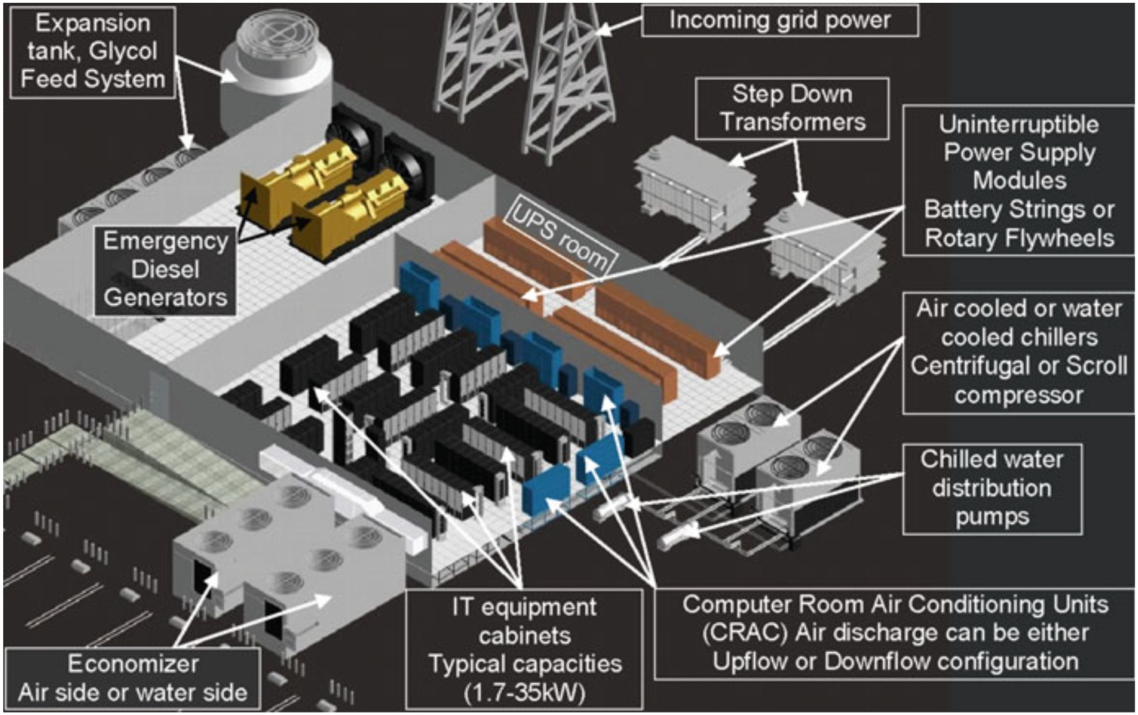
\includegraphics[width=0.65\textwidth]{../figures/joshi2021introduction-figure-01-01.pdf}
%			\vspace{-0.5cm}
		 \caption{(Figure 1.1 in Ref. \cite{joshi2012energy}).}
		\end{figure}
\end{frame}
}

{
\setbeamertemplate{background}{} % Hides background for this frame
\setbeamertemplate{footline}{}   % Reclaims the bottom space
\smallframetitle
\begin{frame}
	\frametitle{Seminar 2}
		\begin{itemize}
			\item Dr. David Geb, Synopsys (formerly Ansys)
			\item Title: TBD
			\item Date: Tuesday, 9/29/26
			\item Time: 15:30 (Berkeley Time)
			\item Location: GSPP 150
%			\item It will be recorded and posted to bCourses. Please do not distribute. 
		\end{itemize}
\end{frame}
}

{
\setbeamertemplate{background}{} % Hides background for this frame
\setbeamertemplate{footline}{}   % Reclaims the bottom space
\smallframetitle
\begin{frame}
	\frametitle{Project 2}
	
In Project 2, you will analyze airflow within the data hall using CFD. You will develop airflow handling strategies. You will use Cadence Reality DC Design Pro.

\end{frame}
}

{
\setbeamertemplate{background}{} % Hides background for this frame
\setbeamertemplate{footline}{}   % Reclaims the bottom space
\smallframetitle
\begin{frame}
	\frametitle{\href{https://datahub.berkeley.edu/user-redirect/git-pull?repo=https://github.com/mtsn-lab/me137-237a&subPath=examples/cfdThermalTransportEquation.ipynb}{Temperature formulation of the first law of thermodynamics}}

This derivation comes from Ref.\cite{bejan2004convection}.


\end{frame}
}

{
\setbeamertemplate{background}{} % Hides background for this frame
\setbeamertemplate{footline}{}   % Reclaims the bottom space
\smallframetitle
\begin{frame}
	\frametitle{\href{https://datahub.berkeley.edu/user-redirect/git-pull?repo=https://github.com/mtsn-lab/me137-237a&subPath=examples/cfdFiniteDifferenceBuoyancyCavity2.ipynb}{Finite Difference: Buoyance-driven Cavity}}
		\begin{figure}
			
\includegraphics[width=0.5\textwidth]{../figures/2D-buoyancy-driven-cavity-finite-difference.pdf}
%			\vspace{-0.5cm}
		 \caption{Compare with Figures 7.8 and 7.17 from Ref.\cite{ferziger2002computational}.}
		\end{figure}

\end{frame}
}

%{
%\setbeamertemplate{background}{} % Hides background for this frame
%\setbeamertemplate{footline}{}   % Reclaims the bottom space
%\smallframetitle
%\begin{frame}
%	\frametitle{ASHRAE Standards}
%		\begin{itemize}
%			\item Read Only versions of ASHRAE standards can be accessed here: \href{https://www.ashrae.org/technical-resources/standards-and-guidelines/read-only-versions-of-ashrae-standards}{link}.
%			\item See: Standard 90.4-2025 -- Energy Standard for Data Centers. 
%			\begin{itemize}
%				\item Read: mechanical load component (MLC) and electrical loss component (ELC). It regulates the efficiency of the systems that serve the data center (cooling and electrical distribution) and not the IT equipment itself.
%				\item PUE is used to report, but MLC and ELC must be used to comply. 
%			\end{itemize}
%			\item All non-data center spaces in the building must demonstrate compliance with ASHRAE Standard 90.1-2025 (see \href{https://www.energycodes.gov/comcheck}{COMcheck}).
%		\end{itemize}
%\end{frame}
%}



%{
%\setbeamertemplate{background}{} % Hides background for this frame
%\setbeamertemplate{footline}{}   % Reclaims the bottom space
%\smallframetitle
%	\begin{frame}
%		\frametitle{Energy analysis of heat transfer from a cabinet}
%			\begin{itemize}
%				\item In addition to maintaining the inlet air temperatures, data centers also need to adhere to the humidity levels specified by ASHRAE guidelines.
%				\item ASHRAE: American Society of Heating, Refrigerating and Air-Conditioning Engineers
%				\item The relevant technical committee is: TC 9.9 (Mission Critical Facilities, Data Centers, Technology Spaces and Electronic Equipment): The flagship committee for data centers. TC 9.9 sets global industry standards for thermal guidelines. 
%				\item Standard 90.1-2025 -- Energy Standard for Data Centers: \href{https://ashrae.iwrapper.com/ASHRAE_PREVIEW_ONLY_STANDARDS/STD_90.4_2025}{Link}. You need to register in order to read. You can also become a student member of ASHRAE. There is a Golden Gate chapter. 
%		\end{itemize}
%	\end{frame}
%}

%{
%\setbeamertemplate{background}{} % Hides background for this frame
%\setbeamertemplate{footline}{}   % Reclaims the bottom space
%\smallframetitle
%\begin{frame}{The ideal vapor-compression refrigeration cycle}
%  \begin{columns}
%    \begin{column}{0.48\textwidth}
%		\begin{figure}
%			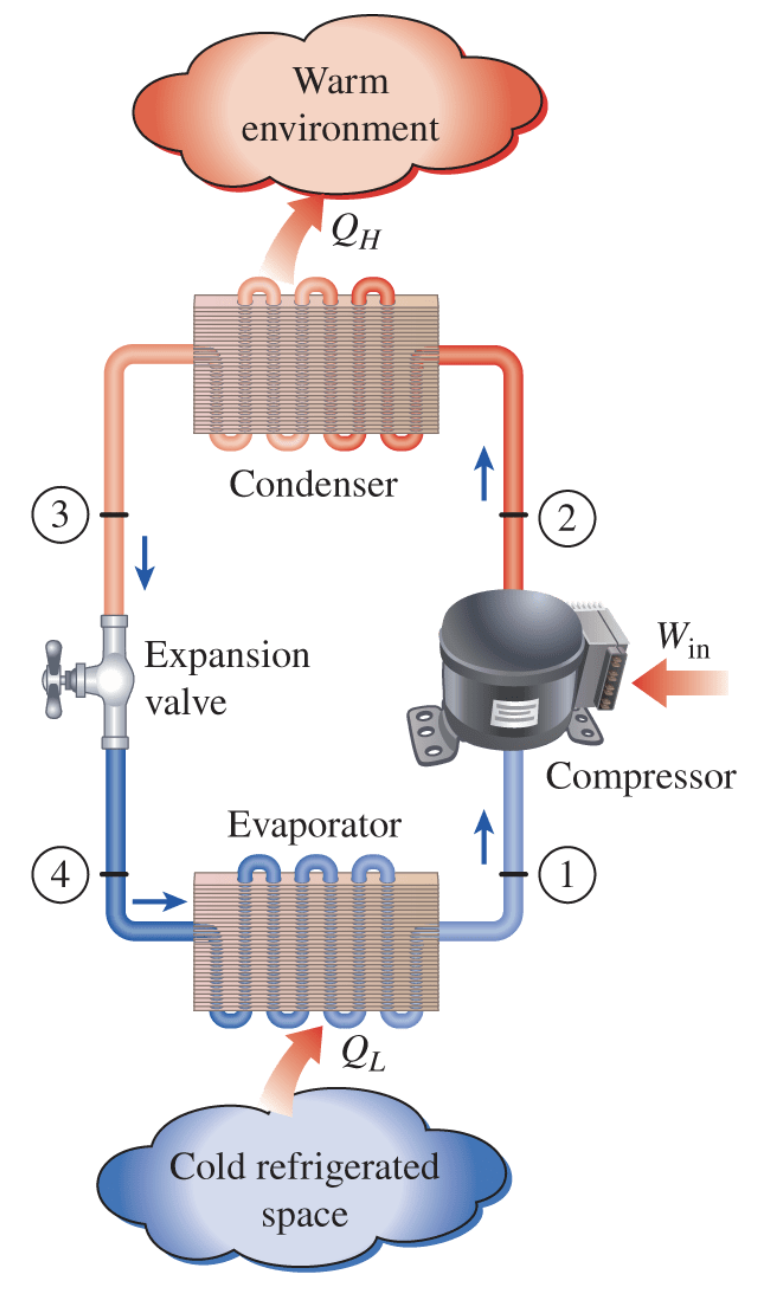
\includegraphics[width=0.5\textwidth]{../figures/cengel2019thermodynamics-figure-11-3.png}
%%			\vspace{-0.5cm}
%		 \caption{\label{fig:refrigeration-system}Reproduced from Figure 11.3 in Ref. \cite{cengel2019thermodynamics}.}
%		\end{figure}
%    \end{column}
%
%    \begin{column}{0.48\textwidth}
%		\begin{figure}
%			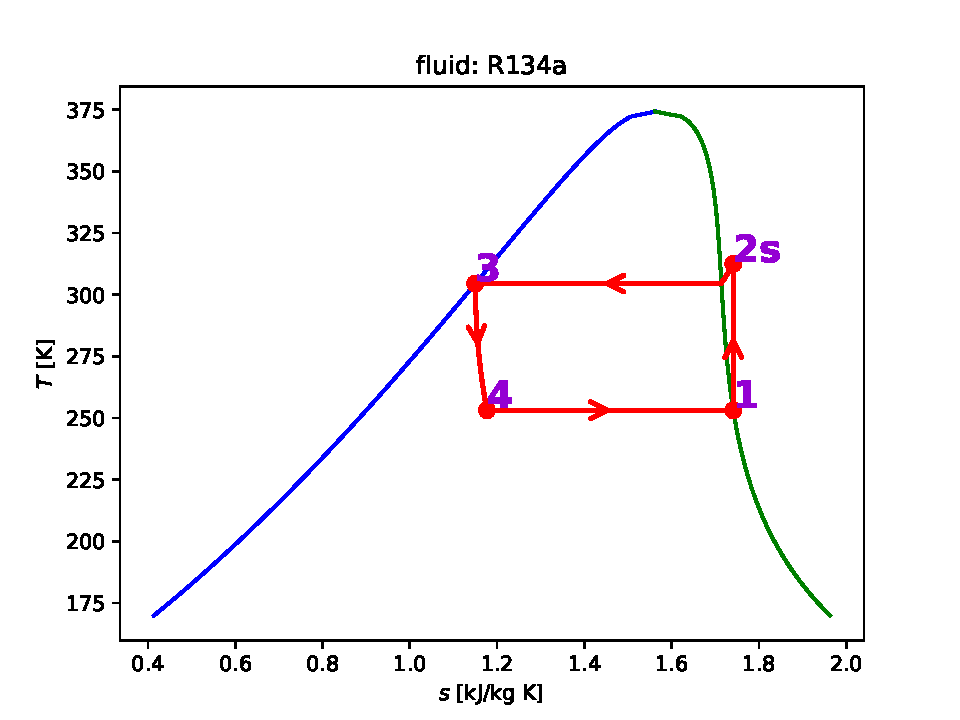
\includegraphics[width=1\textwidth]{../figures/refrigerationCycleR134a_Ts.pdf}
%%			\vspace{-0.5cm}
%		 \caption{\label{fig:refrigeration-system}Generated from \href{https://datahub.berkeley.edu/user-redirect/git-pull?repo=https://github.com/mtsn-lab/me40&subPath=scripts/refrigerationCycleR134a.ipynb}{here}.}
%		\end{figure}
%    \end{column}
%  \end{columns}
%\end{frame}
%}



{
\setbeamertemplate{background}{} % Hides background for this frame
\setbeamertemplate{footline}{}   % Reclaims the bottom space
\setbeamertemplate{bibliography item}[text] % Replaces default icons with numbers
\smallframetitle
	\begin{frame}[allowframebreaks]{References}
		\bibliographystyle{plain}
		\bibliography{../../bibliography}
	\end{frame}
}

%{
%\setbeamertemplate{background}{} % Hides background for this frame
%\setbeamertemplate{footline}{}   % Reclaims the bottom space
%\smallframetitle
%\begin{frame}
%\frametitle{Teaching team}
%
%\begin{columns}[T]
%
%\begin{column}{0.48\textwidth}
%\small
%Ben Brown
%
%		\begin{figure}
%			
\includegraphics[width=0.5\textwidth]{figures/ben-brown.pdf}
%			\vspace{-0.5cm}
%%		\caption{\label{fig:ben-brown}\href{https://eta-publications.lbl.gov/sites/default/files/2024-12/lbnl-2024-united-states-data-center-energy-usage-report.pdf}{eta-publications.lbl.gov}}
%		\end{figure}
%
%
%\end{column}
%
%\begin{column}{0.48\textwidth}
%Amelia Stacey
%
%		\begin{figure}
%			
\includegraphics[width=0.5\textwidth]{figures/oski.jpeg}
%			\vspace{-0.5cm}
%%		\caption{\label{fig:ben-brown}\href{https://eta-publications.lbl.gov/sites/default/files/2024-12/lbnl-2024-united-states-data-center-energy-usage-report.pdf}{eta-publications.lbl.gov}}
%		\end{figure}
%\end{column}
%
%\end{columns}
%\end{frame}
%}




\end{document}
